% =============================================================================
% sections/design/drone/perception_navigation/localization_navigation.tex  -  Localization and Autonomous Navigation Pipeline
% Teams: drone / Status: has placeholder (scope approximation)
%
% EXAMPLE CONTENT for scope/layout approximation - not final report text.
% Scope covers sensor fusion, autonomous search, marker localization, and
% precision landing. Marked with \exampleflag on its heading in the assembler.
% =============================================================================

During the Droning Sub-Task, the Drone operates autonomously using the
architecture shown in \autoref{fig:drone_navigation_dataflow}. The companion
computer manages mission logic and vision processing, while the flight
controller performs pose estimation, stabilization, and command execution.
Detected anomalies activate the corresponding failsafe procedure described in
\autoref{sec:safety}.

The Extended Kalman Filter (EKF) combines IMU and optical-flow data. GPS provides global positioning
for geofence enforcement, while optical flow supports stable local positioning for navigation.
The measured localization performance was
\emph{[Placeholder: provide position error, test conditions, reference ground
truth, and number of trials]}.

After take-off, the Drone follows an outward search pattern until the
downward-facing camera detects the ArUco landing marker. The companion computer
estimates the marker pose, transforms it into the Drone local frame using the
camera calibration and flight-controller orientation, and generates alignment
and descent commands. This allows the system to transition from local-based
area navigation to vision-guided precision landing without operator input.

\todo[inline]{Populate placeholder with the measurements}

\begin{figure}[!htbp]
    \centering
    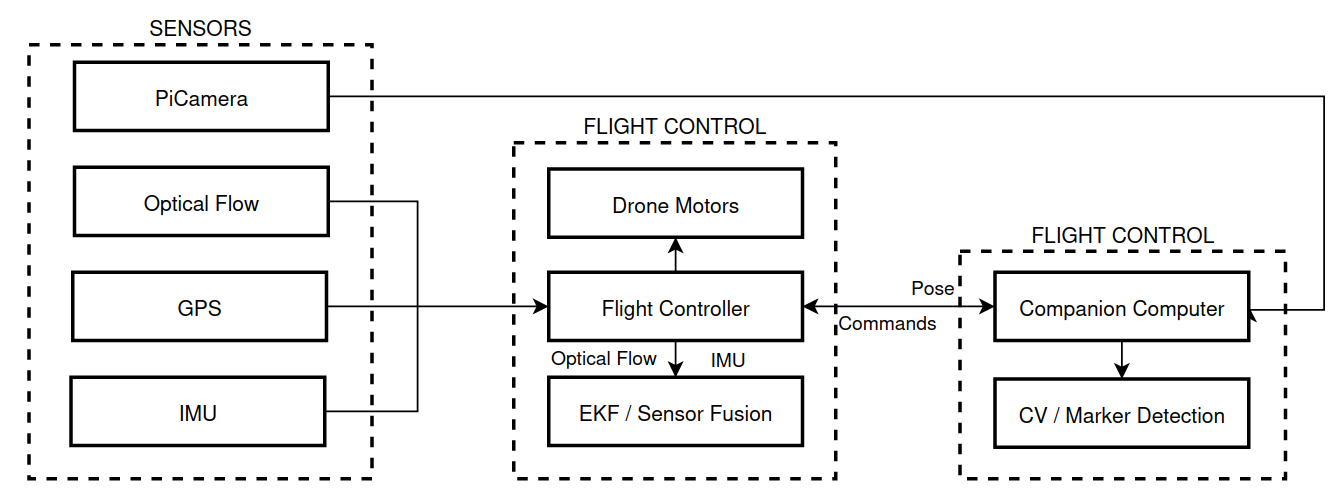
\includegraphics[width=0.7\linewidth]
        {teams/drone/figures/drone_navigation_dataflow}
    \caption{Drone dataflow and control architecture for autonomous
             navigation and task execution}
    \label{fig:drone_navigation_dataflow}
\end{figure}
